
\chapter{Generating Text from Models}


\section{Introduction}

An important transformation involves turning data into text. The text
may be program code, HTML, XML, natural language, or some other format.
The output may be an end in itself (for example documentation) or
may be an intermediate format ready to be processed by a tool (for
example HTML or program code) or may be a save format (for example
XML). Many modelling tools provide support for \textit{code templates}
that allow models to be transformed to program code. These are a special
case of a model to text transformation.

Often, text is generated by running over the data producing standard
chunks of text (or \textit{boiler plate}) with data inserted at appropriate
points. For example, when producing HTML, there will usually be a
standard header and standard components of table definitions.

This chapter describes a language construct that allows text to be
conveniently produced from models. Furthermore, the construct makes
it possible to dip in-and-out of the model and the text interleaved
to any depth, making it easy to structure the transformation so that
it reflects the text as seen in the output.


\section{Examples}

Consider the following operation that expects a class as an argument
and produces a table definition:

\begin{lstlisting}
@Operation classToTable(c)
(1)  @Table(stdout,7)
(2)    table <c.name> {
(3)      // Table for <c.path()>
(4)      <@For a in c.attributes do
(5)        [ field <a.name> : <a.type.name>;
(6)        ]
(7)       e_nd> 
(8)    }
(9) end
end
\end{lstlisting}Line (1) introduces a text transformation of type Table. In general
a text transformation produces literal text interspersed with text
generated by arbitrary bits of XOCL program. Each text transformation
differs in terms of the delimiters used to start and end the literal
text and the XOCL programs. In the case of Table, the delimiters are
<, >, {[} and ].

The arguments used by Table in line (1) are an output channel (to
send the text to) and an integer that indicates where the left margin
should start. In the example, the left margin starts at position 7:
when generating text, whitespace characters up to position 7 are ignored;
or, put another way, everything is left-shifted by 7 characters.

Line (2) starts with some literal text (table) that is sent to the
output channel. Then the \textit{drop} delimiters < and > are encountered.
The drop delimiters surround XOCL code that produces some text to
be sent to the output channel. In this case, the name of the supplied
class is generated. Line (2) concludes with more literal text.

Line (3) is a mixture of literal text (a comment) and the path of
the supplied class. Line (4) introduces a dropped XOCL expression:
a for-loop. Each attribute of the class c produces some text in lines
(5-6) which are surrounded by \textit{lift} delimiters {[} and ].
The lift delimiters are used within a dropped expression to surround
literal text. It should be noted that lifts and drops can be arbitrarily
interleaved.

Lines (5-6) produce text output that describes each of the attributes
in turn. Note that the newline at the end of line (5) is part of the
output.

Line (7) completes the dropped for-loop. Note that normally an XOCL
for-loop is termined by an end keyword. Within a dropped expression,
end cannot be used since it will confuse the lifting mechanism (as
explained below), so the convention is to use e\_nd within lifted
text. The only end-keyword that is permitted must be that at the end
of the outermost lifted text -- line (9).

In review, the Table construct is an example of a model to text template.
The body of the template is literal text, up to an open drop delimiter.
The text inside the drop delimiter, up to the corresponding closing
drop delimiter, is XOCL code (containing e\_nd instead of end where
necessary). The dropped XOCL code can do anything, but should return
a string that is dropped into the surrounding literal text of the
template. Within dropped XOCL code, literal text can be used surrounded
by lift delimiters. The lift delimiters surround a model to text template
(just like Table), however, nested templates can use the delimiters
rather than the @TemplateName ... end notation. Drops and lifts can
be nested to any depth, and in general the actual delimiters used
to demote the lift and drop can be defined (so that they do not clash
with literal text used in the body of the template). Newlines within
lifted text are carried through to the output with the left hand margin
affected by the initial value supplied to the template (7 in the example
above).

Supplying Class to the Table template produces the following:

\begin{lstlisting}
table Class {
  // Table for Root::XCore::Class
  field attributes : Set(Attribute);
  field isAbstract : Boolean;
  field constructors : Seq(Constructor);
}
\end{lstlisting}Notice how the literal text in the lifted parts has been copied through
verbatim, whereas the name of the class and the names of the attributes
have been dropped into the text. The following example shows how drops
and lifts can be interleaved to good effect. The aim is to produce
an HTML page containing the description of a class. The attributes
of the class are to be rendered as a table; each row of the table
describes an attribute: the first row is the name of the attribute
and the second row is the name of the attribute's type.

\begin{lstlisting}
@Operation classToHTML(class:Class,out:OutputChannel)
  @HTML(out,4)
    <HTML>
      <HEAD>
        <TITLE> {class.name} </TITLE>
      </HEAD>
      <FONT SIZE="+2">
        <B> { class.name } </B>
      </FONT>
      <BR><BR><HR>
      <FONT SIZE="+1">
        <B>Overview</B>
      </FONT>
      <BR>
      <P> {c.doc().doc}
      <BR><HR><BR>
      <FONT SIZE="+1">
        <B>Parents:</B>
      </FONT>
      { @For p in class.allParents() do
          [ { p.name.toString() } ]
        e_nd }
      <BR><HR><BR>
     <TABLE WIDTH="100%" CELLPADDING="3" CELLSPACING="0">
        <TR BGCOLOR="#CCCCFF" CLASS="TableHeadingColor">
          <TD COLSPAN=3>
            <FONT SIZE="+2">
              <B>Attributes</B>
            </FONT>
          </TD>
        </TR>
        { @For a in class.attributes do
           [ <TR>
               <TD>
                 <B> {a.name.toString()} </B>
               </TD>
               <TD>
                 <B> { a.type.name().toString() } </B>
               </TD>
             </TR>
           ]
         e_nd
       }
     </TABLE>
   </HTML>
  end
end
\end{lstlisting}%
\begin{figure}
\begin{center}

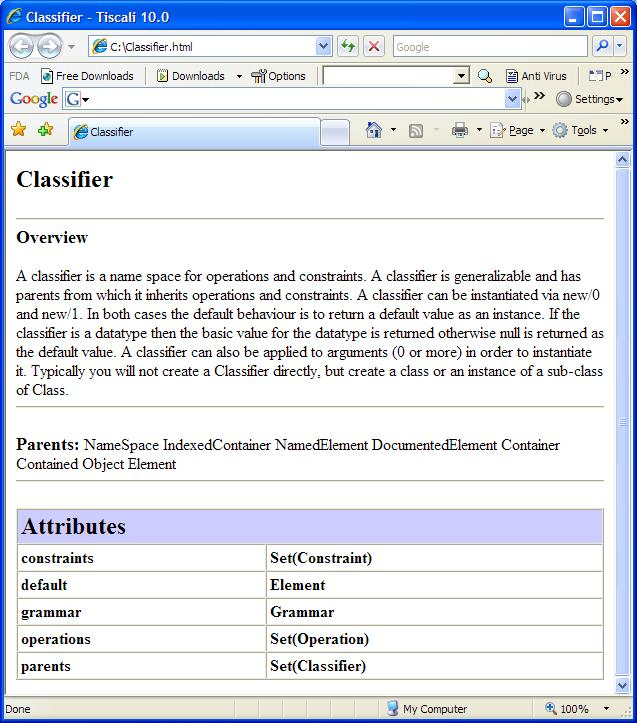
\includegraphics[width=12cm]{LanguageEngineering/TextFromModels/Images/Classifier}

\caption{G\label{fig:Generating-HTML}enerating HTML}

\end{center}
\end{figure}


In classToHTML notice how the table rows for each attribute are priduced
by a dropped for-loop. The body of the for-loop is a lifted table-row,
where the attribute name and type are dropped in. This interleaving
is typical of the template mechanism. Notice how the structure of
the required output is retained (i.e. an HTML page) where the model
data is dropped in at appropriate points. The HTML page for the class
Classifier is viewed in a web browser as shown in figure \ref{fig:Generating-HTML}.


\section{Specification}

Code templates can be implemented as a transformation into XOCL code.
Each element of the text in a template is turned into a format statement.
Literal text ets turned into a format statement that just prints out
the text. Dropped expressions are transformed into format statements
that evaluate the expressions and then print out their results. The
complications arise from keeping track of the indentation and from
the interleaving of lifts and drops.

To understand how the transformation works it is useful to look at
a few examples. Suppose we have a construct X that is defined to be
a template:

\begin{lstlisting}
@X(out,0)
  Some text.
end
\end{lstlisting}is translated to the following code:

\begin{lstlisting}
// Output spaces...
format(out,"~V",Seq{3});
// Output the text...
format(out,"Some text.")

If newlines are included in the text then they are faithfully recreated
in the output:

\begin{lstlisting}
@X(out,0)
  Some 
    text.
end
\end{lstlisting}produces the following code...

\begin{lstlisting}
// Output spaces...
format(out,"~V",Seq{3});
// Output the text...
format(out,"Some");
// Newline and pad to the appropriate column...
format(out,"~%~V",Seq{5});
format(out,"text.")
\end{lstlisting}Now, suppose that a simple expression is dropped into the middle...

\begin{lstlisting}
@X(out,0)
  Some { dropped } text.
end
\end{lstlisting}The output should include the value of the variable named 'dropped'
in between the literal text for {}``Some'' and {}``text.''. Therefore
the code that is produced looks like the following:

\begin{lstlisting}
// Pad to the appropriate column...
format(out,"~V",Seq{3});
// Output the literal...
format(out,"Some "});
// Get the value of dropped and check
// that it is a string. If so then
// print it...
let str = dropped
in if str.isReallyKindOf(String)
   then format(out,str)
   end
end;
// The rest of the literal output...
format(out," text.")
\end{lstlisting}Within a dropped expression it is possible to introduce a lifted literal:

\begin{lstlisting}
@X(out,0)
  Some { dropped1 [ then lifted ] dropped2 } text.
end
\end{lstlisting}What we would like to achieve for the nested lifting is the following:

\begin{lstlisting}
format(out,"~V",Seq{3});
format(out,"Some "});
let str1 = dropped1
in if str1.isReallyKindOf(String)
   then format(out,str1);
        format(out," then lifted ");
        let str2 = dropped2
        in if str2.isReallyKindOf(String)
           then format(out,"str2)
           end
        end
   end
end;
format(out," text.")
\end{lstlisting}Note that the nested lift, is equivalent to another occurrence of
@X ... end, therefore we could just produce the following code:

\begin{lstlisting}
format(out,"~V",Seq{3});
format(out,"Some "});
let str = dropped1
in if str.isReallyKindOf(String)
   then format(out,str)
   end
end;
@X(out,3) then lifted end;
let str = dropped2
in if str.isReallyKindOf(String)
   then format(out,str)
   end
end;
format(out," text.")
\end{lstlisting}Now we have a general rule for dealing with nested lifts: just wrap
the nested lift up in the appropriate template construct (passing
in the current margin for indentation). This will deal with any level
of nesting and interleaving:

\begin{lstlisting}
@X(out,0)
  Some { dropped1 [ then { nested } lifted ] dropped2 } text.
end
\end{lstlisting}Is translated to:

\begin{lstlisting}
format(out,"~V",Seq{3});
format(out,"Some "});
let str = dropped1
in if str.isReallyKindOf(String)
   then format(out,str)
   end
end;
@X(out,3) then { nested } lifted end;
let str = dropped2
in if str.isReallyKindOf(String)
   then format(out,str)
   end
end;
format(out," text.")
\end{lstlisting}which in turn becomes:

\begin{lstlisting}
format(out,"~V",Seq{3});
format(out,"Some "});
let str = dropped1
in if str.isReallyKindOf(String)
   then format(out,str)
   end
end;
format(out," then ");
let str = nested
in if str.isReallyKindOf(String)
   then format(out,str)
   end
end;
format(out," lifted ");
let str = dropped2
in if str.isReallyKindOf(String)
   then format(out,str)
   end
end;
format(out," text.")
\end{lstlisting}
\section{Design}

In order to perform the transformation from a template to code, we
must keep track of the level of nesting. This can be done using a
simple two-state transition machine. the machine is wither currently
lifting or is currently dropping. At each stage the machine consumes
input characters until it receives a lifting or dropping token. When
it receives a token it changes state. The machine builds literals,
lifts and drops. Each time a literal character is encountered it is
added to the literal currently being constructed. When the machine
encounters an end token, it constructs an appropriate element (either
a lift or a drop) and consumes the literal tokens. When the machine
encounters a start-token (either lift or drop) then it changes state
and starts a new collection of literals:

%
\begin{figure}
\begin{center}

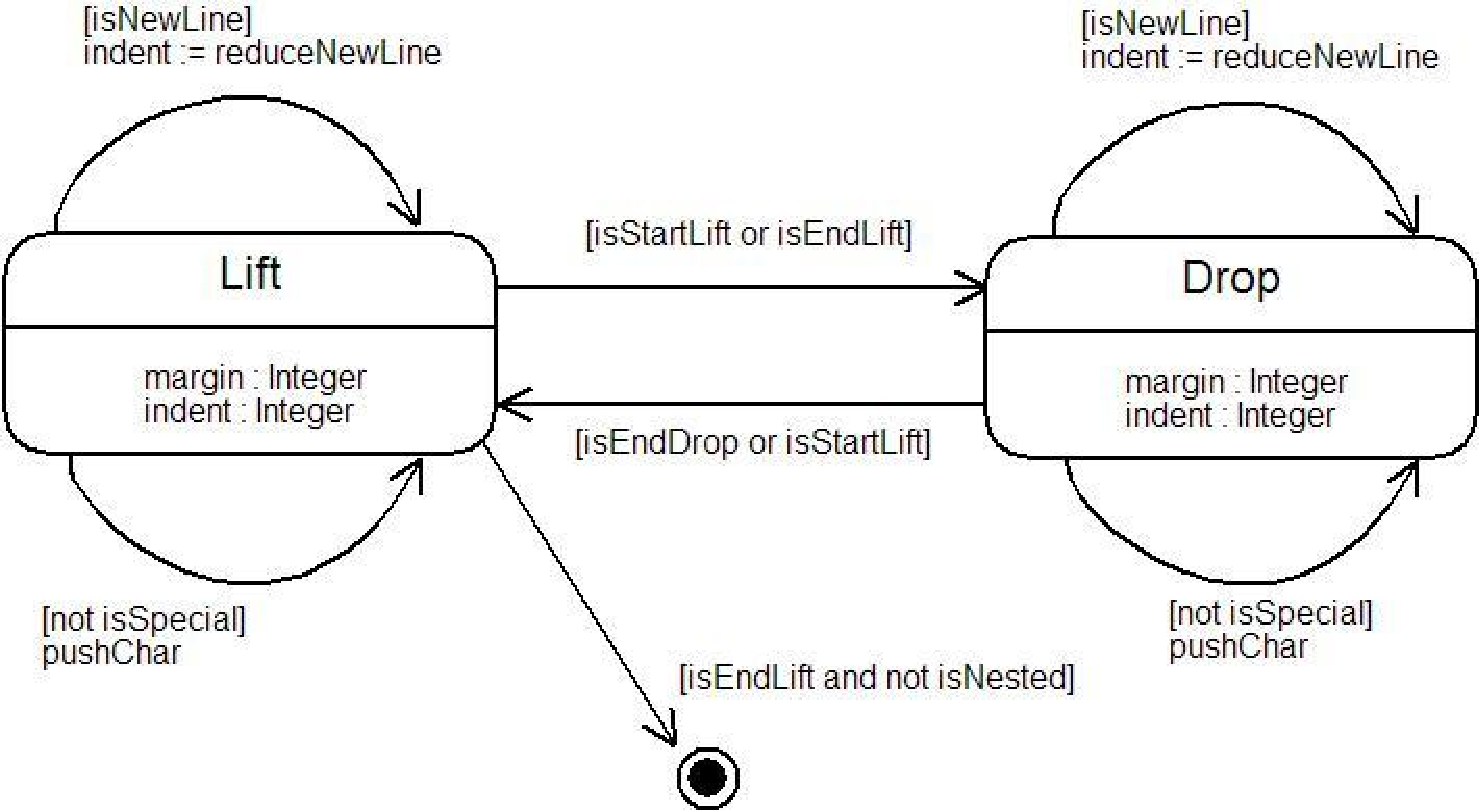
\includegraphics[width=12cm]{LanguageEngineering/TextFromModels/Images/StateMachine}

\caption{L\label{fig:Lift-and-Drop}ift and Drop Mechanism}

\end{center}
\end{figure}


The state machine consumes an input string and produces a code element
that represents the structure of the template. The model of code elemnts
is shown below:

%
\begin{figure}
\begin{center}

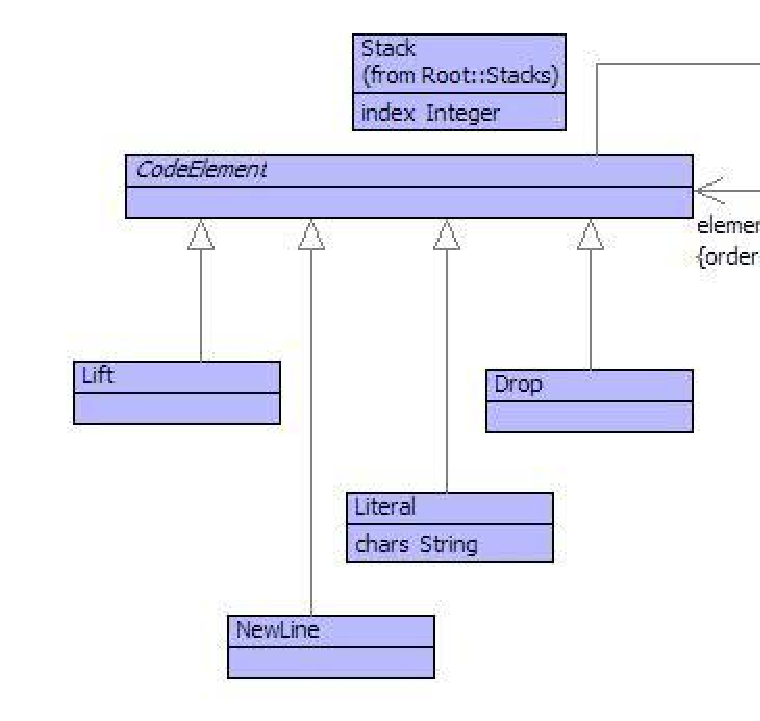
\includegraphics[width=12cm]{LanguageEngineering/TextFromModels/Images/CodeElement}

\caption{Code Elements}

\end{center}
\end{figure}


A code element is a literal string containing text that is to be printed
on the output channel. Code elements retain newlines so that the indentation
can be controlled. The structure of lift and drop blocks in a template
is retained by constructing instances of Lift and Drop. An lift or
drop object contains a sequence of code elements produced by translating
the input string in between the start and end tokens.

For example, the template:

\begin{lstlisting}
@X(out,0)
  Some text.
end
\end{lstlisting}produces the following code elements when processed by the state machine:

\begin{lstlisting}
Lift(0,Seq{
  NewLine(0,3),          
  Literal(Some text.),          
  NewLine(0,1),          
  Literal()
})
\end{lstlisting}Note that the NewLine instances contain two values. The first value
is the amount to left-shift all input. This value is supplied to the
template as the argument after the output channel. In the example,
@X(out,0) ... end supplied 0 as the adjustment to the left-hand margin.

The following example includes further newlines:

\begin{lstlisting}
@X(out,0)
  Some 
    text.
end
\end{lstlisting}and produces the following code elements:

\begin{lstlisting}
Lift(0,Seq{          
  NewLine(0,3),          
  Literal(Some),          
  NewLine(0,5),          
  Literal(text.),          
  NewLine(0,1),          
  Literal()
})
\end{lstlisting}Dropped text becomes wrapped in an instance of Drop:

\begin{lstlisting}
@X(out,0)
  Some { dropped } text.
end
\end{lstlisting}is translated into the following instance by the state machine:

\begin{lstlisting}
Lift(0,Seq{       
  NewLine(0,3),
  Literal(Some ),
  Drop(Seq{
    Literal( dropped )
  }),
  Literal( text. )
})
\end{lstlisting}Finally, if we interleave drops and lifts then these are faithfully
reproduced in the code element structure:

\begin{lstlisting}
@X(out,0)
  Some { dropped1 [ then { nested } lifted ] dropped2 } text.
end
\end{lstlisting}becomes:

\begin{lstlisting}
Lift(0,Seq{
  NewLine(0,3),
  Literal(Some ),
  Drop(Seq{
    Literal( dropped1 ),
    Lift(2,Seq{
      Literal(then ),
      Drop(Seq{
        Literal( nested )
      }),
      Literal( lifted )
    }),
    Literal( dropped2 )
  }),
  Literal( text.)
})
\end{lstlisting}
\section{Implementation}

A code template is implemented as a language construct that is defined
in terms of tokens for the start and end of lift and drop respectively.
The language construct grammar simply consumes all the text in between
the start of the template and the keyword 'end'. The text is then
loaded onto the machine and the machine is executed to produce a code
element. The code element is then transformed into abstract syntax
that is the returned by the grammar. Here is an example template:

\begin{lstlisting}
@Class X extends CodeGen::Generator
    @Grammar extends OCL::OCL.grammar
      X ::= 
        '(' // Get the output channel... 
            out = Exp 
            // get the current level of indent...
            ',' indent = Int 
        ')'     
        // Get the raw text...   
        s = Char*   
        'end'            
         { let // The control tokens for the code generator...
               startLift = "[";
               endLift = "]";
               startDrop = "{";
               endDrop = "}";  
               // All references to 'end' are protected...   
               protectEnd = s.asString().subst("end","e_nd",true) then   
               // All references to newline characters are protected...   
               protectNewline = protectEnd.subst("\n","\\n",true) then
               newString = startLift + protectNewline + endLift then
               // Create the mapping to a code element...
               mapping = Mapping(newString,startLift,endLift,startDrop,endDrop) then
               // Perform the mapping (run the machine) ...
               lift = mapping.processLift(indent,indent)    
           in 
              // Translate the code element to abstract syntax and return...
              lift.desugar("CodeGen::X",
                startLift,endLift,startDrop,endDrop,startExtract,endExtract,out,0) 
           end
       }.       
    end
\end{lstlisting}In the example template X defined above, the start- and end-lift tokens
are {[} and ] respectively, and the start- and end-drop tokens are
\{ and \} respectively. Note how the keyword 'end' replaces occurrences
of the keyword 'e\_nd' before the machine is performed. Including
XOCL code in templates must use the keyword 'e\_nd' instead of 'end'
in order that the transation does not get confused.

The mapping is loaded with the token information and the input string.
Notice how the input text (protectNewline) is loaded onto the machine
by surrounding it with the start- and end-lift tokens. This is because
the main body of the template is equivalent to an outermost 'lift'. 

The machine is executed with respect to the following state:

\begin{lstlisting}
@Class Mapping
    // The input string...
    @Attribute chars        : String end
    // The stack of code elements being generated...
    @Attribute stack        : Stack = Stack() end
    // The current position in the string...
    @Attribute index        : Integer end
    // The token indicating a start lift...
    @Attribute startLift    : String end
    // The token indicating the end of a lift...
    @Attribute endLift      : String end
    // The token indicating the start of a drop...
    @Attribute startDrop    : String end
    // The token indicating the end of a drop...
    @Attribute endDrop      : String end
    // The constructor...
    @Constructor(chars,startLift,endLift,startDrop,endDrop) end
    ...
\end{lstlisting}The machine constructs values on a stack. At any given time there
is a sequence of code elements being built at the head of the stack.
To support this, the machine arranges for the head element of the
stack to be another stack onto which the current sequence of code
elements are pushed. The following operations manipulate the stack:

\begin{lstlisting}
context Mapping
    @Operation pushChar()
      // Elements are added to the top-stack. Generally
      // the head element is a buffer. The next literal
      // char is added to the top-buffer...
      let elements = stack.top() then
          b = elements.top()
      in b.add(chars->at(index));
         self.index := index + 1
      end
    end
context Mapping   
    @Operation pushElement(element)
      // Add an element to the top-stack...
      let elements = stack.top()
      in elements.push(element)
      end
    end
context Mapping
    @Operation reduceDrop()
      // An end-drop has been consumed. The top-stack
      // contains the elements to be dropped...
      let elements = stack.pop().asSeq()
      in Drop(elements)
      end
    end
context Mapping         
    @Operation reduceLift()
      // An end-lift has been encountered. The top-stack
      // contains the elements to be lifted...
      let elements = stack.pop().asSeq()
      in Lift(elements)
      end
    end
context Mapping         
    @Operation reduceLit()
      // The literal being constructed at the head of the
      // top-stack has terminated. The buffer is replaced
      // by a literal...
      let elements = stack.top() then
          b = elements.pop() then
          str = b.toString()
      in elements.push(Literal(str))
      end
    end
context Mapping    
    @Operation reduceNewLine()
      // When new-lines are encountered in the template
      // they are retained in the code-element so that
      // indentation can be manipulated...
      self.reduceLit();
      self.index := index + 1;
      let whiteSpace = self.skipWhiteSpace()
      in stack.top().push(NewLine(margin,whiteSpace));
         self.restart();
         whiteSpace
      end
    end
context Mapping   
    @Operation restart()
      // Create a new empty literal buffer in a
      // sequence of existing code-elements...
      let elements = stack.top()
      in elements.push(Buffer(10,true))
      end
    end
context Mapping
    @Operation start()
      // Start a completely new sequence of code-elements...
      let elements = Stack()
      in stack.push(elements);
         self.restart()
      end
    end
\end{lstlisting}The machine needs to recognize when the current position in the input
corresponds to one of the tokens. a number of token predicates are
implemented. All token recognition predicates follow the same basic
implementation which is shown as follows:

\begin{lstlisting}
context Mapping
  @Operation hasPrefix(p:String):Boolean
    // Returns true when the current input starts 
    // with the token p...
    let hasPrefix = true;
        i = index
    in @While hasPrefix and not i = chars->size and (i - index) < p->size do
         hasPrefix := chars->at(i) = p->at(i - index);
         i := i + 1
       end;
       hasPrefix
    end
  end
context Mapping
  @Operation isStartLift():Boolean
    // Returns true when the next token is start-lift...
    self.hasPrefix(startLift)
  end
\end{lstlisting}The machine is implemented using two main operations: processLift
and processDrop. Each operation defines the state-machine processing
that occurs when the machine is in the corresponding state. The first
operation that is called is processLift (since the complete template
corresponds to an outermost lift):



\begin{lstlisting}
@Operation processLift()
  // Advance past the start-lift token...
  self.consumeStartLift();
  // Until we get to the end of this lift...
  @While not self.isEndLift() do
    if self.isNewLine()
    then 
      // Record the newline...
      self.reduceNewLine()
    elseif self.isStartDrop()
    then 
      // A nested drop is to be processed.
      // Any literal text is consumed...
      self.reduceLit();
      // Change state...
      self.processDrop();
      // Prepare to carry on with the lift...
      self.restart()
    else 
      // Consume a literal character...
      self.pushChar()
    end
  end;
  // Advance past the end-lift token...
  self.consumeEndLift();
  // Consume the most recent literal...
  self.reduceLit();
  // Build a lift from the tokens on the
  // stack...
  self.reduceLift()
end
\end{lstlisting}The implementation of processdrop is very similar, however it uses
different tokens:

\begin{lstlisting}
@Operation processDrop(margin,indent0,indent)
   self.consumeStartDrop();
  @While not not self.isEndDrop() do
    if self.isNewLine()
    then self.reduceNewLine()
    elseif self.isStartLift()
    then
      self.reduceLit(); 
      self.processLift();
      self.restart()
    else self.pushChar()
    end
  end;
  self.consumeEndDrop();
  self.reduceLit();
  self.reduceDrop()
end
\end{lstlisting}The code elements produced by the machine are translated into XOCL
code. As we have seen in the design, outer-most literals are simply
formatted to the output channel. Nested drops are translated to XOCL
code that evaluates an expression to produce a string and then formats
the string to the output channel. Lifts that are nested within drops
are translated to templates are re-processed using the machine. The
re-processing is now at the outermost level and therefore produces
XOCL code. 

The processing is implemented using two code element operations: desugar
and dropString. The outermost Lift instance is sent a 'desugar' message
in order to produce the XOCL code:

\begin{lstlisting}
context Lift    
  @Operation desugar(path:String,
                     lstart:String,
                     lend:String,
                     dstart:String,        
                     dend:String,
                     out:Performable,
                     nesting:Integer):Performable
    // The arguments are the name-space path to the template
    // the tokens, the output channel and the level of nesting.
    // Desugar the lifted elements. Lifting an element produces code,
    // each code element will produce some string output when it is
    // executed...
    elements->iterate(e code = [| null |] |
      [| <code>; 
         // Add 1 to the level of nesting...
         <e.desugar(path,lstart,lend,dstart,dend,out,level+1)> 
      |])
  end
\end{lstlisting}Desugaring a literal or a new-line is straightforward:

\begin{lstlisting}
context Literal
  @Operation desugar(path:String,lstart,lend,dstart,dend,out,level):Performable
    [| format(<out>,"~S",Seq{<chars.lift()>}) |]
  end

context Newline
  @Operation desugar(path:String,lstart,lend,dstart,dend,out,level):Performable
    [| format(<out>,"~%~V",Seq{<(indent - base).lift()>}) |]
  end
\end{lstlisting}Desugaring an instance of Drop involves inserving the code for the
dropped expression and then printing the resulting string to the output
channel at run-time. The literals in between the start of the drop
and the end of the drop is to be viewed as XOCL code. Therefore we
must construct a string containing the code, then turn the string
into XOCL code by parsing it. Code elements can be transformed into
strings ready for the XOCL parser using the 'dropString' operation
as called in the following operation:

\begin{lstlisting}
context Drop
  @Operation desugar(path:String,lstart,lend,dstart,dend,out,level):Performable
      // Turn the elements into code. The elements are strings that
      // are concatenated to produce XOCL code that is parsed using 
      // the OCL grammar...
      let str = elements->iterate(e s = "" | 
                  s + e.dropString(path,out,lstart,lend,dstart,dend,0)) then
          code = OCL::OCL.grammar.parseString(str,"Exp1",Seq{XOCL})
      in [| let s = <code>
            in if s.isReallyKindOf(XCore::String)
               then format(<out>,s)
               end
            end
         |]
      end
    end
\end{lstlisting}Now we need to implement 'dropString' for each of the code element
classes. The result from 'dropString' must be a string that corresponds
to the XOCL code for the element. Literals and Newlines are straightforward:

\begin{lstlisting}
context Literal
  @Operation dropString(path:String,out,lstart,lend,dstart,dend,level):String
    // Careful to replace outermost ocurrences of e_nd in user code with
    // end...
    if level = 0
    then chars.subst("end","e_nd",true)
    else chars
    end
  end
context Newline
  @Operation dropString(path:String,out,lstart,lend,dstart,dend,level):String       
    "\n" + formats("~V",Seq{indent})     
  end
\end{lstlisting}A Lift is dropped by transforming it into a template construct:

\begin{lstlisting}
context Lift
  @Operation dropString(path:String,out,lstart,lend,dstart,dend,,level):String
    // Dropping a lift with respect to the level of nesting. If the
    // level is 0 then the lift and drop cancel out and we produce the
    // code as a string (ready to splice into surrounding code)...
    if level = 0  
    then
      "@"+path+"(" + out.pprint() + "," + margin + ") " + 
         elements->iterate(e s = "" | 
           s + e.dropString(path,out,lstart,lend,dstart,dend,level+1)) + 
      " end"
    else 
      lstart + 
        elements->iterate(e s = "" | 
          s + e.dropString(path,out,lstart,lend,dstart,dend,level+1)) + 
      lend
    end
\end{lstlisting}Finally, a Drop generates a drop string by wrapping itself with drop
start- and end-tokens:

\begin{lstlisting}
context Drop
  @Operation dropString(path,out,lstart,lend,dstart,dend,level):String
    
    // To create a string from a drop. Wrap it with the 
    // drop-start and drop-end tokens...
      
    dstart + elements->iterate(e s = "" | 
      s + e.dropString(path,out,lstart,lend,dstart,dend,level)) + 
    dend
  end
\end{lstlisting}
